\section{Ablations}
\label{sec:ablation}

The ablation asks a narrower question than the main comparison: on a single long task that the baseline never closes, which change makes closure possible? All arms use MiniMax-M3.1-Flash on the same tabulate formatting issue, on one machine with one key, run in sequence. We organise the result as four hypotheses; Appendix~\ref{app:debuglog} reproduces the run order and the per-arm cost of each step.

\paragraph{Hypothesis one: capacity.} If the episode fails because it runs out of room, then removing the pressure should let it finish.
We made three capacity interventions in turn: evicting repeated reads, raising the share of the budget available to file reads, and raising the session token ceiling.
The observations did not move. Deduplicating repeated reads left the count at 0/3\fact{E2}; enlarging the read share left it at 0/3\fact{E3}; raising the ceiling left it at 0/2\fact{E4}.
The starting point, with the card assembled but not delivered and with no gate, was 0/3\fact{E1}.
Each intervention removed a defect in the transcript and left an episode that could not terminate, so capacity was not the variable.

\paragraph{Hypothesis two: instruction.} If the episode fails because the model does not know the procedure, then stating the procedure should fix it.
We wrote the required process as six constraints --- deliver a patch early, do not re-read a span, note a conclusion before acting, stay in scope, hand in rather than test, keep output short --- and assembled them as resident project-rule sections, ordered after the charter and before the task, rendered into the system message.
The count stayed at 0/3\fact{E5}, and per-turn output grew rather than shrank.
The rules were read and treated as a description of the situation rather than as a procedure: adding text to the system prompt changed what the model said about its work, not what the episode did.

\paragraph{Hypothesis three: delivery.} If the evidence is correct but never arrives, then rendering it should move the first read.
We had reported the card as delivered; verifying the recorded request bodies showed that it had not been. Once the card was actually rendered, the first read landed in the gold region on every attempt, and the count moved to 1/4\fact{E6}.
The intervention solved direction and did not solve termination. It also separated delivery from effect: the card is necessary and, on this task, not sufficient.

\paragraph{Hypothesis four: the location of the decision.} If the model will not submit on its own, then the harness should take the decision away.
Moving a reminder into the loop produced patches but no submission: 0/2\fact{E7}. Capping the number of patch versions at two, closing on the second and sending the last version to the verifier, moved the count to 5/5\fact{E8}.
What separates this arm from the ones above is neither more evidence nor a better instruction but the location of the decision: the harness, not the model, decides when the episode ends.

Read as a sequence, the ablation is not a dose-response curve. The early arms each removed a visible defect and left the episode unable to close; the last arm removed a choice. That is why we treat the card as a precondition for the gate rather than as the intervention by itself, and why the mechanism claim is about the gate rather than about the amount of context.

\begin{figure}[t]
\centering
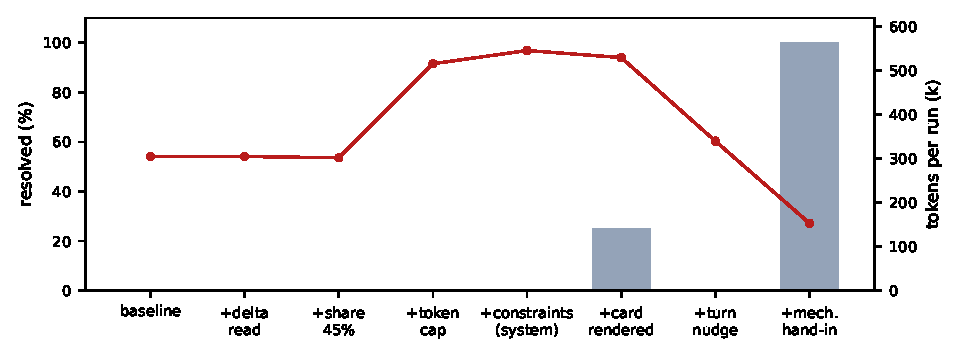
\includegraphics[width=\linewidth]{figures/f1_progression.pdf}
\caption{Incremental ablation on a single task (one tabulate issue, MiniMax-M3.1-Flash).
Each step adds one mechanism: repeated-read deltas, a larger tool-result share, a larger
session budget, prompt-level constraints, an actually-rendered locator card, a mechanical
turn nudge, and mechanical hand-in. Resolved count is the bar; tokens per run the line.
Data: Table~\ref{tab:ablation}; the run order is in Appendix~\ref{app:debuglog}.}
\label{fig:progression}
\end{figure}

% FACTS-USED: E1, E2, E3, E4, E5, E6, E7, E8
